\documentclass[10pt,twocolumn]{article}
\usepackage[letterpaper,margin=0.72in,columnsep=0.24in]{geometry}
\usepackage{graphicx,booktabs,amsmath,amssymb,multirow,array,enumitem}
\usepackage[colorlinks=true,linkcolor=blue,citecolor=blue,urlcolor=blue]{hyperref}
\usepackage{microtype,placeins}
\urlstyle{same}
\setlength{\parindent}{1em}
\setlength{\parskip}{0pt}
\setlength{\textfloatsep}{8pt plus 2pt minus 2pt}
\setlength{\floatsep}{7pt plus 2pt minus 2pt}
\setlength{\intextsep}{7pt plus 2pt minus 2pt}
\renewcommand{\arraystretch}{1.10}
\setlist[itemize]{leftmargin=1.35em,itemsep=2pt,topsep=3pt}
\newcommand{\pFive}{2×5}
\newcommand{\pTen}{2×10}
\newcommand{\srcone}{source column 1}
\title{\vspace{-1em}\textbf{From Visual Rules to Reliable Robot Manipulation:}\\An AI Advisor--Executor Study of Versions V1--V10}
\author{Yicheng Zhao \qquad Sihua Zhang \qquad Ruilin Gao\\[0.15em]
\small Group 3 \quad | \quad AI305 Intelligent Agent Systems and Programming}
\date{\small 9 November 2026}
\begin{document}
\maketitle
\vspace{-1.0em}
\begin{abstract}
\noindent
We built a rule-based controller for the A3 dual-arm cookie-packing simulator and improved it through ten software versions. The robot sees the source and target boxes through cameras, grasps a requested group of cookies, carries it across the workspace, and places it without disturbing the remaining cookies. Rather than learning actions from demonstrations, our controller combines visual measurements, known robot geometry, touch feedback, and a sequence of simple decisions.

A central part of our development process was an \emph{AI advisor--executor loop}: a GPT-6 advisor analyzed failed runs and suggested focused changes; coding agents implemented those changes and ran controlled tests; the human team conveyed evidence and selected the next direction. We preserve successful and unsuccessful versions, matched comparisons, and runnable evaluation code.

The first evaluated milestone (V5) achieved 46.83\% mean task completion and 14.17\% official success. The frozen V10 policy achieved 98.42\% completion and 95.83\% success in one 120-episode test, followed by 96.62\% and 94.17\% on another 120 episodes with newly sampled seeds. These measurements use the benchmark's standard source-column-1 grid.
\end{abstract}
\vspace{-0.4em}
\section{Task and Setting}
\label{sec:task}
Our assignment is a small but demanding robot-packing task in the A3 dual-arm MuJoCo simulator~\cite{a3}. A robot must move thin, closely packed cookies from a \emph{source box} into a \emph{target box}. It must take the correct number of cookies in each grasp and place them neatly without leaving cookies hanging over an edge, knocking over its earlier work, or accidentally dragging extra cookies out of the source.

There are two tasks. In \pFive, the robot transfers two groups of five cookies, making ten target cookies. In \pTen, it makes four transfers: first $n$ cookies, then $10-n$, and repeats that pattern for the second target column. The first-group size $n$ may vary between trials. Thus, \pTen\ is not merely a longer \pFive: the robot must handle a thin single cookie as well as a large group, and the first group affects the space available for later ones.

The source has four columns, each containing twenty cookies. The course's standard six-setting evaluation uses \srcone; the simulator also supports selecting the other three columns. Each task is tested under \emph{Basic}, \emph{Medium}, and \emph{Advanced} scene variation. The environment changes relevant box and cookie positions, camera parameters, lighting, and, for the hardest setting, cookie colors. These changes are applied by the official benchmark, not by our policy.

\paragraph{What the robot can know.}
The policy receives RGB images from a front camera and two wrist cameras, together with public robot motion and gripper/force observations. It can use the known shape of the robot and its fingers. It does not read the simulator's hidden positions of cookies to decide what to do. During development, the evaluator records such hidden information separately, so we can explain a failure after a run without giving the policy an unfair advantage.

\paragraph{What counts as success.}
The teacher's final score uses two complementary measures. \emph{Completion} counts how many cookies end in valid target positions; \emph{success} requires the entire task to satisfy the simulator's placement and source-box conditions. For example, ten cookies may appear to have arrived in \pFive, but disturbing a separate cookie in the source can still make the run unsuccessful. This distinction shaped much of our later work.

\section{The AI Advisor--Executor Workflow}
\label{sec:workflow}
The policy was built in an iterative collaboration between a human team and AI assistants. It is useful to distinguish their roles because the project is about \emph{improving software through experiments}, not training one neural model to control the robot.

\begin{figure*}[t]
\centering
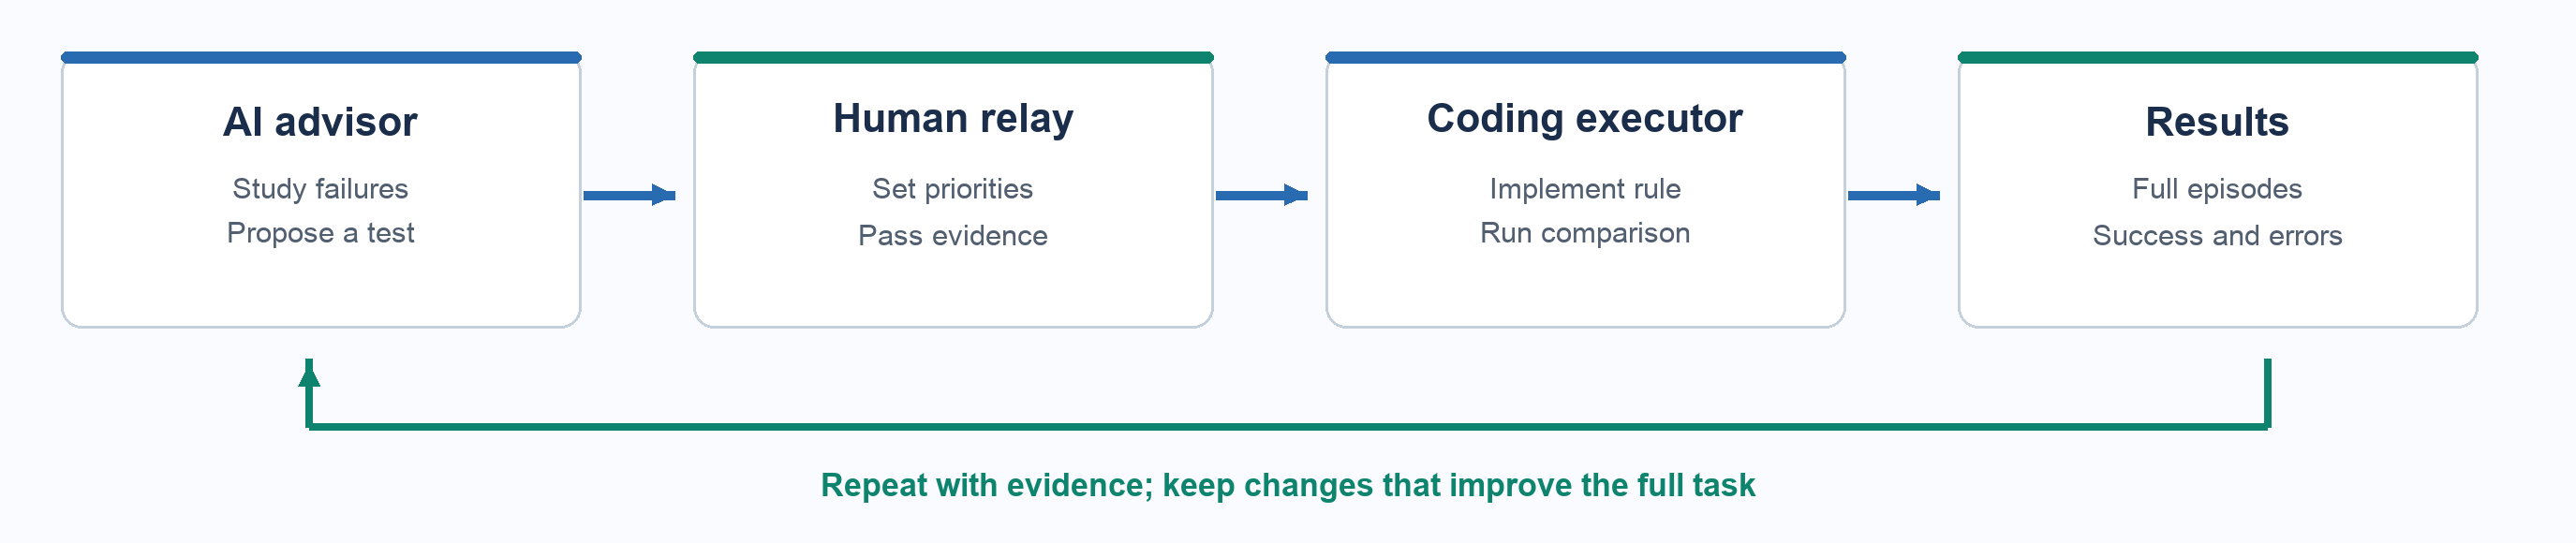
\includegraphics[width=0.99\textwidth]{figures/advisor_executor_loop.png}
\caption{The development loop. The advisor diagnoses and proposes a focused change; the human team relays the plan and sets priorities; a coding executor implements and tests it; the resulting successes and failures guide the next iteration.}
\label{fig:advisor}
\end{figure*}

\paragraph{Advisor: decide what to investigate.}
The advisor was GPT-6 in the Astra configuration. It read run summaries, inspected source code and failure evidence, compared alternative explanations, and proposed concrete experiments. Its main output was a decision such as: \emph{check whether the robot is following an outdated box position before changing the grasp force}. The advisor also decided whether promising small-test changes deserved a larger evaluation and which regressions mattered.

\paragraph{Executor: make and measure the change.}
The coding executors were separate, high-reasoning agent processes, including GPT-6.1 Sol (xhigh), GLM-5.3 (xhigh), and DeepSeek V4 Flash 1017 (high), as available at different stages. They worked on local files and the authorized compute machines. An executor typically read the preceding implementation, modified the Python policy, ran simulator trials, collected errors, and returned results and saved code. This separation let the advisor reason about the overall approach while the executor handled the detailed implementation and repeated tests.

\paragraph{Human team: coordinate and verify.}
Group 3 set the research goal, chose the rule-based approach, transferred plans and results between otherwise separate agent sessions, checked important decisions, and assembled the final submission. In practice, the human often acted as the messenger between advisor and executor. The files exchanged were plans, code locations, experimental outputs, and short summaries rather than a single uninterrupted AI conversation.

\paragraph{One iteration in practice.}
The working cycle had five steps:
\begin{enumerate}[leftmargin=1.45em,itemsep=1pt,topsep=2pt]
\item \textbf{Find the first meaningful failure.} Was a group misidentified, missed during grasp, lost while carrying, or placed incorrectly?
\item \textbf{Write a small, testable explanation.} For instance, the target camera may be seeing an old object position.
\item \textbf{Make one targeted change.} Keep unrelated parts of the controller unchanged.
\item \textbf{Test both failures and previous successes.} Compare the new code with the old version on matched seeds where possible.
\item \textbf{Keep, revise, or discard.} Freeze a version only when its complete-run results justify the change.
\end{enumerate}

This process made a useful distinction between an attractive idea and a successful policy. Some changes solved one visible problem but created another. We kept those negative results and used them to narrow later improvements. Figures~\ref{fig:advisor} and~\ref{fig:controller} illustrate the software-development loop and the robot's own feedback loop, which operate at different time scales.

\section{How the Rule Policy Works}
\label{sec:controller}
At each control step, the policy follows a simple principle: \emph{look at the current scene, decide which part of the job is next, make a small movement, and check what actually happened}. This is a feedback controller rather than a fixed prerecorded motion. Layered feedback control and visual servoing are established ideas in robotics~\cite{brooks,servo}; our work applies them to the particular geometry and scoring rules of this cookie task.

\begin{figure*}[t]
\centering
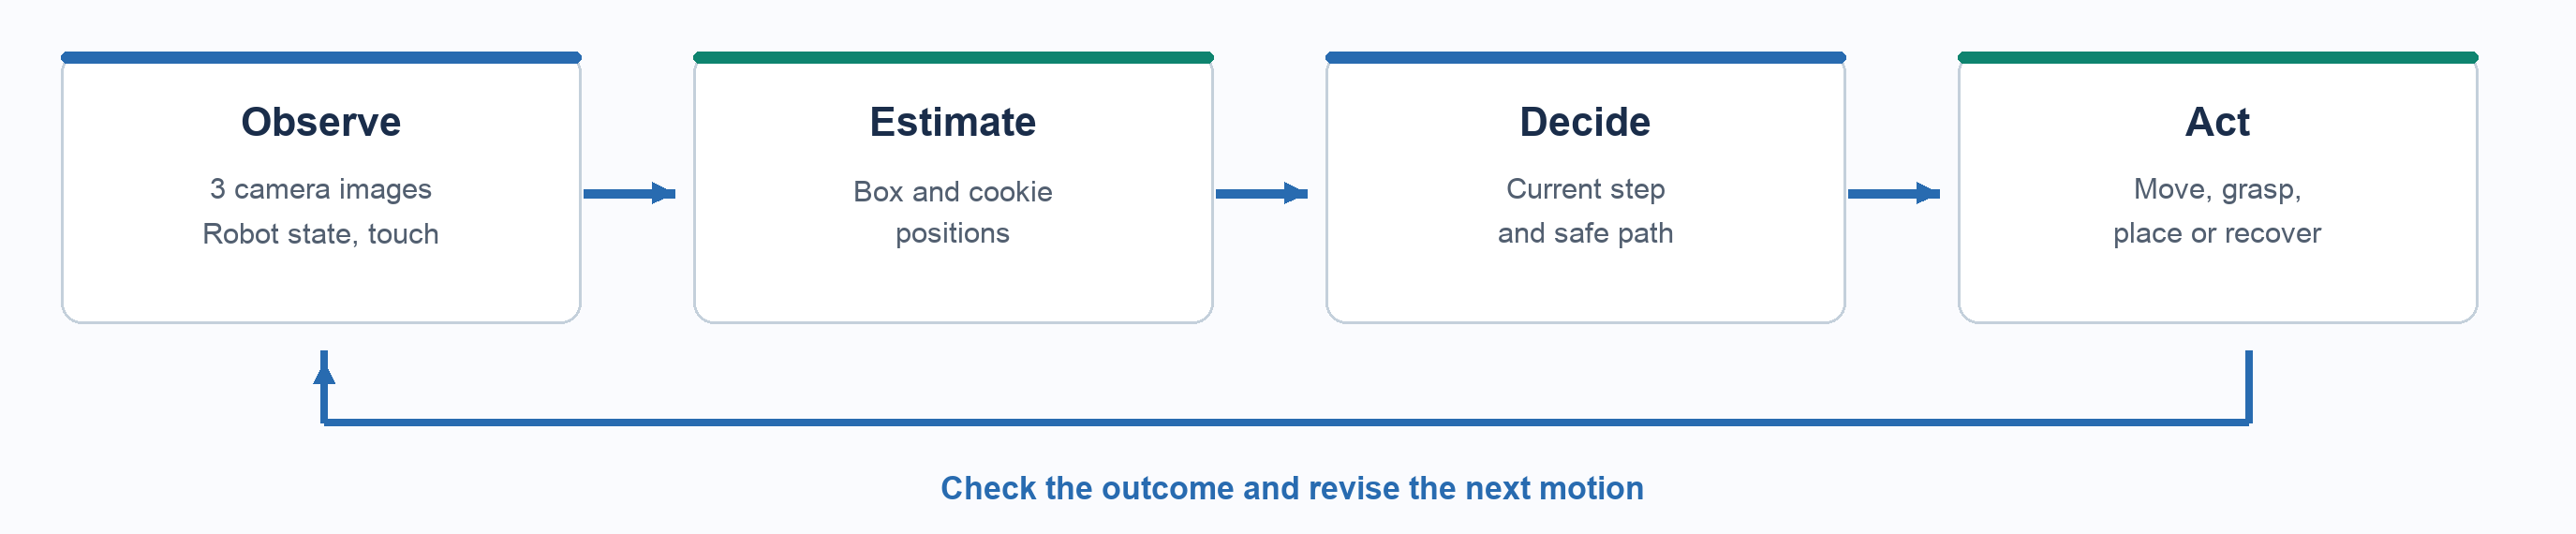
\includegraphics[width=0.99\textwidth]{figures/feedback_controller.png}
\caption{V10's high-level operation. Camera images and public robot measurements are turned into an estimate of the boxes, cookies, and gripper. The controller chooses a movement and checks the next observation before continuing.}
\label{fig:controller}
\end{figure*}

\subsection{Seeing the boxes and the cookies}
The three cameras see different aspects of the same scene. The front view helps locate the source and target boxes; wrist views are useful when the gripper approaches a narrow gap. Our visual estimator uses the known sizes and shapes of the boxes, robot, and cookies to interpret image edges and colored regions. Where the scene changes slightly, it updates the estimated positions rather than relying solely on the initial layout.

This distinction matters at millimeter scale. For example, a cookie may be centered according to the original box coordinates but offset from the actual gap after the camera or box has moved. A small correction at the last moment can decide whether the fingers enter between cookies or push the entire row. We therefore use broad views to find the layout and closer views to refine the final grasp.

\subsection{Moving in understandable stages}
The rule controller keeps track of which step it is performing. Table~\ref{tab:stages} describes the main stages in ordinary terms. There are also short observation and recovery stages when the robot has insufficient evidence to continue safely.

\begin{table}[t]
\centering\small
\caption{The robot's main actions and the feedback used between them.}
\label{tab:stages}
\begin{tabular}{p{1.6cm}p{5.65cm}}
\toprule
Stage & Meaning \\
\midrule
Choose group & Identify the requested number of remaining cookies. \\
Approach & Move the gripper above the group and line it up with the narrow gap. \\
Grasp & Lower the fingers carefully, close them, and check contact. \\
Lift & Raise the group; verify that the cookies followed the gripper. \\
Carry & Move above the target while checking the held group. \\
Place & Lower into a free region, release when supported, and retreat. \\
Check & Confirm progress; if needed, reobserve, correct, or retry. \\
\bottomrule
\end{tabular}
\end{table}

The controller uses robot geometry to convert desired gripper movement into feasible arm motion. In the final release, it returns the simulator's \emph{Cartesian delta} action: a small change in end-effector position, orientation, and gripper command, rather than an image or a neural-network prediction.

\subsection{Checking contact and carrying}
The first motion after closing the fingers is a cautious lift. Images and force signals help the controller distinguish a real grasp from fingers touching a nearby surface. While carrying, it estimates the group relative to the gripper. If the group slips, the robot should not continue toward a target position calculated for the old grip.

A useful example occurred during development: the robot visibly picked up cookies but carried them about 2--3\,mm away from the assumed position. The same error could later place one edge on the target rim. We addressed such failures by checking the \emph{held object as it is}, not just the gripper pose that was requested.

\subsection{Making room for the next group}
A successful placement has two parts. The current group must fit inside the target, and the robot must be able to open its fingers and withdraw without hitting earlier cookies. In \pTen, the first placement must also leave a reasonable route for the second group. V8--V10 increasingly accounted for these neighboring objects and the changing target layout instead of treating each drop as independent.

This is where several common failures came from: a place looked empty in one view but was blocked by previously placed cookies; an old image was used after the box moved; or the gripper could approach a nominal target point but had no safe way to retreat. The policy therefore links placement decisions to the space occupied by the \emph{whole held group and fingers}, not only to the center of a cookie.

\subsection{Remembering progress and recovering}
The controller tracks the requested batch sizes and how much of the job appears complete. When observations disagree, it may take a better view or return to an earlier step. Later versions added more careful handling of unknown outcomes, a moved box, and a group that was lifted or placed imperfectly.

For example, if a group has already arrived near the target, repeatedly returning to the source to pick it again can create an error. Conversely, counting a group as placed merely because the fingers opened can miss cookies resting on an edge. An explicit account of the groups, their likely locations, and the remaining planned work is essential to deciding the next action.

\paragraph{Why use rules here?}
The task provides well-defined objects and known robot geometry. This lets us express many actions directly: where the fingers should go, when to move slowly, what a safe approach looks like, and when the visual evidence is too weak. The policy is interpretable: a failed run can often be traced to a wrong visual estimate, an unsafe movement, or an incorrect stage transition. Improving these pieces is the focus of the next section.

\section{Building and Improving V1--V10}
\label{sec:development}
Our main tool for improvement was to observe \emph{where} a run first went wrong. A final count of five cookies does not say whether the remaining five were never grasped, lost during carrying, or placed in the wrong location. Each explanation calls for a different change. The advisor therefore requested stage-by-stage evidence; the executor tested a small fix and returned both successful and unsuccessful examples.

\subsection{V1--V5: from a basic idea to a tested policy}
The first four versions were development prototypes. They established the basic pipeline rather than a benchmark result for every version.

\paragraph{V1: a first closed-loop routine.}
We began with a geometric description of the robot, boxes, and expected cookie arrangement. The first controller estimated the scene from camera images and followed a sequence of approach, grasp, lift, carry, and release. It was capable of issuing real robot actions, but relied heavily on the nominal positions of the groups.

\paragraph{V2: look at the selected group.}
A broad estimate of all cookies was not enough for narrow grasping. We added a closer estimate of the actual group and a visual count of objects held between the fingers. This addressed two different questions: \emph{where should the gripper close?} and \emph{how many cookies did it take?}

\paragraph{V3: check camera alignment.}
A camera estimate can shift the perceived cookie position even when the robot motion is correct. We added a way to refine the front-camera alignment from visible source-box geometry. This aimed to reduce errors shared by all later steps.

\paragraph{V4: also inspect the target.}
A successful grasp is only half the job. The controller gained a target-side cookie count so that it could judge whether placement had made progress. This prepared the ground for later placement checks.

\paragraph{V5: first full frozen evaluation.}
V5 combined these pieces into a version that we tested on 20 seeds for each of six task/variation settings. Its mean completion rate was \textbf{46.83\%}, and official success was \textbf{14.17\%} (17/120). The failure logs were especially useful: the fingers often missed a narrow gap, failed to lift the entire group, or placed a partially held group against the target edge. Increasing the allowed action budget alone yielded little additional success, so the next versions focused on the quality of the movements.

\subsection{V6: use feedback where precision matters}
V6 was the largest early step forward. The executor worked on more accurate wrist-camera alignment, correct gripper-opening geometry, held-cookie measurements, and simpler recovery when a movement did not reach its goal. The advisor used small trials to identify errors in each stage before approving a wider evaluation.

One particularly useful result came from comparing two approaches to checking placement. A less restrictive version, which continued after reasonable visual evidence and kept uncertainty visible, succeeded in \textbf{19 of 45} development episodes. A version that insisted on strong visual confirmation before nearly every transition succeeded in only \textbf{3 of 45}. The stricter version often stopped because the camera could not see enough, even when movement was physically possible. We chose the less restrictive approach and retained the strict checker as diagnostic information.

In the paired 120-episode comparison at seeds 15000--15019, completion rose from \textbf{42.88\% to 74.58\%} and success from \textbf{5.83\% to 48.33\%}. This result gave a clear direction: improve local sensing and contact handling while allowing the robot to keep moving when it has sufficient evidence.

\subsection{V7: distinguish a helpful correction from a harmful one}
The next round targeted target-box localization and the last few millimeters of alignment. Some episodes improved sharply when the controller rejected an incorrect target estimate. However, the same correction sometimes displaced a previously successful approach. We tested reduced versions of the change instead of simply adding more recovery rules.

The paired comparison at seeds 16000--16019 found that V7 raised completion from \textbf{65.12\% to 67.38\%}, but official success changed from \textbf{36.67\% to 33.33\%}. This was a mixed result. We kept the improved observation and alignment ideas and carried the regressions into subsequent testing. The experience changed our review criterion: final quantity and official success had to be considered together, with specific attention to cases that were correct before a change.

\subsection{V8: separate the two tasks and handle the next move}
The two packing tasks need different handling. With ten cookies, the second group may be very small or very large, and the first group can block the next placement. V8 made it easier to give the two tasks distinct planning rules, observe the remaining source group after a change, and check the space that the moving fingers actually need.

An earlier controller could repeatedly attempt the same grasp without noticing that its information was stale. Another could choose a target point that was inside the box while the fingers could not safely withdraw. V8 began to address these task-level failures rather than treating them only as motion errors.

In the matched 17000-series evaluation, completion improved from \textbf{74.33\% to 81.21\%} and success from \textbf{45.00\% to 50.83\%}. The parent in this particular comparison was a composed candidate built from the previous work, not simply the published V7 folder. We preserved the exact parent and candidate code in the history archive.

\subsection{V9: make repeated pick-and-place reliable}
V9 focused on the long \pTen\ sequences. The most important lesson from the preceding runs was that correct motion on the first group did not guarantee progress on the third or fourth. The world had changed: a cookie had moved, an empty gap had appeared, or the target already contained a neighboring group.

The advisor proposed more specific source observations, clearer accounting of the remaining groups, better use of the visible box edges, and a distinction between a group that was physically in the target and one that passed every final scoring condition. Executors tested variations, measured regressions, and updated the controller only after a complete-run comparison.

A representative failure showed why this matters. After one group had been moved, the controller could continue searching for cookies in their old source position. More observation steps did not automatically help; the controller needed to update \emph{what had moved} and \emph{what still had to be done}. V9 improved this connection between observation, inventory, and the next action.

On seeds 19000--19019, V8 achieved \textbf{76.46\%} completion and \textbf{47.50\%} success; V9 achieved \textbf{88.12\%} completion and \textbf{75.00\%} success on those same settings. This established a more effective base for the final round.

\subsection{V10: selective fixes, then freeze}
For V10 we did not replace everything. We treated the six task/source cases as related but distinct problems and selected code that worked for each one. Important improvements included more reliable detection of the target box and already placed cookies, source-group re-identification after moving objects, more careful use of carried-object shape in collision checking, and better handling of a difficult final group.

A concrete example came from a source group that was carried successfully but also pulled an additional neighboring cookie. Although twenty cookies could appear in the target, the source-box condition still failed. This shifted our attention from merely increasing target count to protecting the remaining source cookies. Another example involved a target region mistakenly considered occupied because an old observation was reused. The solution was to revisit the evidence for that region, not blindly relax collision checks.

We also deliberately rejected changes that looked good on a few cases. A broad sideways correction briefly helped a four-case test. On a larger 127-case comparison it produced both new successes and \emph{fourteen lost previous successes}, with a small decrease in the total number of valid cookies. We did not merge this global correction into V10. Instead, we kept the stronger, better-tested components and used the failed examples to guide future targeted fixes.

The final V10 release is a frozen set of \textbf{78 policy runtime files}. We verified their hashes before formal testing. On seeds 24000--24019, the same-scene V9 baseline reached \textbf{94.96\%} completion and \textbf{89.17\%} success, while V10 reached \textbf{98.42\%} and \textbf{95.83\%}. Its final deployment uses the original task instructions and official scoring.

\begin{figure*}[t]
\centering
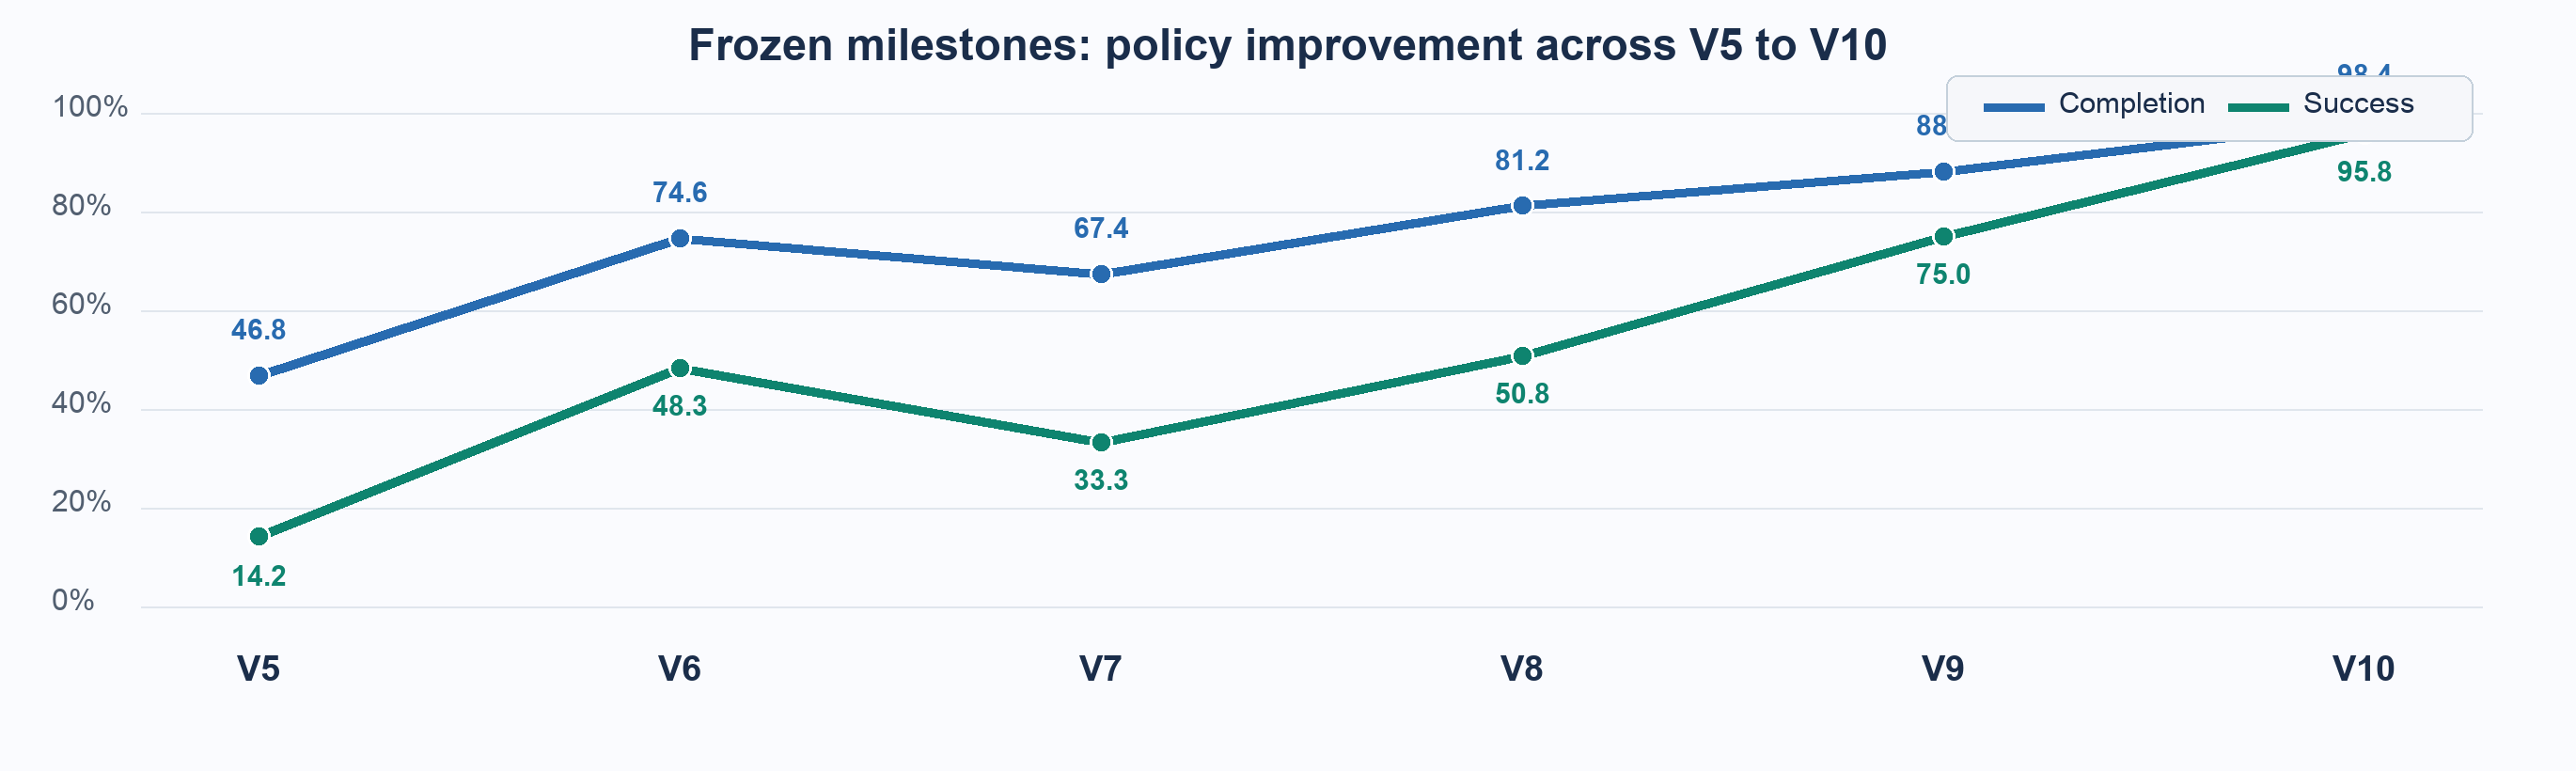
\includegraphics[width=0.99\textwidth]{figures/milestones.png}
\caption{The main milestones from V5 to V10, each measured on a newly chosen development or formal evaluation set. Values are mean completion and official success. Because the test scenes differ by round, Table~\ref{tab:paired} gives the more informative same-scene changes. The dips are retained rather than smoothed away.}
\label{fig:milestones}
\end{figure*}

\begin{table*}[t]
\centering\small
\caption{Same-scene comparisons used during selection. Each comparison has 120 episodes (20 seeds per setting); figures are mean completion and official success. Positive changes reflect paired improvements, while the V7 row illustrates a regression in one metric.}
\label{tab:paired}
\setlength{\tabcolsep}{3.7pt}\footnotesize\begin{tabular}{llrrrrrr}
\toprule
Test seeds & Old → new & Old completion & New completion & Change & Old success & New success & Change \\
\midrule
15000--15019 & V5 → V6 & 42.88\% & 74.58\% & +31.71 pp & 5.83\% & 48.33\% & +42.50 pp \\
16000--16019 & V6 → V7 & 65.12\% & 67.38\% & +2.25 pp & 36.67\% & 33.33\% & -3.33 pp \\
17000--17019 & Composed base → V8 & 74.33\% & 81.21\% & +6.88 pp & 45.00\% & 50.83\% & +5.83 pp \\
19000--19019 & V8 → V9 & 76.46\% & 88.12\% & +11.67 pp & 47.50\% & 75.00\% & +27.50 pp \\
24000--24019 & V9 → V10 & 94.96\% & 98.42\% & +3.46 pp & 89.17\% & 95.83\% & +6.67 pp \\
\bottomrule
\end{tabular}
\end{table*}

\paragraph{Our decision rule.}
Across these versions, a change was valuable when it improved complete tasks and did not needlessly spoil cases already handled well. We preferred small changes with a clear explanation to larger sets of emergency rules. A strong result on one scene could motivate a test, but wider same-scene comparisons decided whether it belonged in the frozen policy.

\section{Evaluation and Results}
\label{sec:evaluation}
\subsection{What we measure}
We use the benchmark's two final metrics. If episode $i$ asks for $m_i$ cookies and the official scorer counts $c_i$ valid target cookies, its completion is $c_i/m_i$. The reported mean completion and mean success are
\begin{equation}
\label{eq:metrics}
C=(c_1/m_1+\ldots+c_N/m_N)/N,
\qquad S=(s_1+\ldots+s_N)/N.
\end{equation}
Here $s_i$ is 1 for an officially successful episode and 0 otherwise. Both numbers are averaged \emph{per episode}. Each of the six task/settings has twenty episodes, so the overall result also equals the equal-weight mean of the six settings. We additionally publish raw cookie counts, which are helpful for checking the arithmetic.

The evaluator uses the task's original stopping and scoring rules. The \pFive\ budget is 500 robot control steps; \pTen\ has 3,200. A complete success must satisfy the official conditions for five consecutive steps. Both tests use non-strict mode, which preserves each task's own release requirements. The policy sees three cameras, the public robot state, and the task instruction; the evaluator alone determines the official score.

\subsection{Two independent test batches}
The final code was frozen before the first test, and we used the \emph{same} code for the second test.

\paragraph{Test A: initial holdout.}
Twenty seed values, 24000--24019, were chosen in advance. We ran both tasks in all three variation levels, giving $20\times2\times3=120$ episodes. This is the same test used to compare V9 and V10 in Table~\ref{tab:paired}.

\paragraph{Test B: additional random seeds.}
A separate re-evaluation drew twenty distinct values from 620000--620999 using Python's random sampling, before running any of those episodes. The list is published in the repository. Again we ran the full six-setting grid, giving another 120 episodes. Both were run with the official simulator and CPU software rendering. The source column was 1 in both tests, while the scene's configured position, view, color, and lighting changes were sampled as usual.

\begin{table*}[t]
\centering\small
\caption{Frozen V10 performance on two independent sets of 20 seeds. Each row contains 20 episodes in each test. Completion uses the final valid cookie count; success uses the original simulator flag. The second test is the new 620xxx-seed reproduction.}
\label{tab:holdouts}
\begin{tabular}{llrrrrrr}
\toprule
& & \multicolumn{3}{c}{Test A: seeds 24000--24019} & \multicolumn{3}{c}{Test B: 20 new random seeds}\\
\cmidrule(lr){3-5}\cmidrule(lr){6-8}
Task & Variation & Cookies & Completion & Success & Cookies & Completion & Success\\
\midrule
\multirow{3}{*}{\pFive} & Basic    & 200/200 & 100.00\% & 20/20 & 195/200 & 97.50\% & 19/20\\
 & Medium   & 200/200 & 100.00\% & 20/20 & 200/200 & 100.00\% & 20/20\\
 & Advanced & 200/200 & 100.00\% & 20/20 & 190/200 & 95.00\% & 19/20\\
\midrule
\multirow{3}{*}{\pTen} & Basic    & 380/400 & 95.00\% & 18/20 & 400/400 & 100.00\% & 20/20\\
 & Medium   & 400/400 & 100.00\% & 19/20 & 391/400 & 97.75\% & 19/20\\
 & Advanced & 382/400 & 95.50\% & 18/20 & 358/400 & 89.50\% & 16/20\\
\midrule
\textbf{Mean} & \textbf{120 episodes each} & \textbf{1762/1800} & \textbf{98.42\%} & \textbf{115/120} &
 \textbf{1734/1800} & \textbf{96.62\%} & \textbf{113/120}\\
\bottomrule
\end{tabular}
\end{table*}

\subsection{What changed, and what repeated}
Table~\ref{tab:holdouts} shows that V10 performs consistently well on two separate collections of randomized scenes. The first test gave \textbf{98.42\% mean completion} and \textbf{95.83\% success}; the second gave \textbf{96.62\% completion} and \textbf{94.17\% success}. Pooling both equal-sized test batches gives \textbf{97.52\% mean completion} and \textbf{95.00\% success} across 240 evaluated episodes.

The \pFive\ task was particularly reliable: 60/60 successes in Test A and 58/60 in Test B. For \pTen, both tests happened to give exactly 55/60 successes. The second test was strongest in Basic \pTen\ (20/20) and weakest in Advanced \pTen\ (16/20). This is consistent with the difficulty of keeping all parts of a large transfer aligned when vision and object positions vary.

The new seed sample also provides concrete failed cases rather than only a single average: for example, seed 620335 affected both Basic and Advanced \pFive, while seed 620780 affected Medium and Advanced \pTen. All seven failed episodes from Test B ended at the allowed control-step limit. These episodes remain in the published results; their purpose is to help reviewers see what is still difficult.

\subsection{Why the gain is meaningful}
The important improvement is not just the final percentage. Earlier versions often had a visible problem, a plausible rule change, and no reliable way to know whether the change helped the whole task. By V10, we routinely compared a candidate against its parent on \emph{the same seed and task setting}, while keeping the camera, object randomization, scoring rules, and run budget consistent within each comparison.

For the final V9-to-V10 comparison, mean completion increased by 3.46 percentage points and success by 6.67 points on matched seeds. The separate 620xxx test then reproduced the same overall level of performance with an entirely new set of randomized scenes. Together, these results support the development decisions better than a collection of handpicked successful demonstrations.

\paragraph{Evaluation scope.}
The official six-setting grid fixes the requested source at column 1. The underlying simulator supports columns 2--4 as well. Our open repository includes the multi-column branches and development evidence; the numerical headline here reports the exact grid that was tested twice.

\section{How Much Computation Does the Policy Need?}
\label{sec:latency}
High task success and fast computation are different goals. We therefore compared V10 with the teacher's released SmolVLA checkpoint using a separate timing experiment. The question was simple: once camera images and robot measurements are available, how long does each policy take to return its next action?

\subsection{A comparison on the same recorded inputs}
We recorded every control step of two V10 runs: a Basic \pFive\ episode with 316 steps and an Advanced \pTen\ episode with 671 steps. Both used source column 1 and development seed 19000; the latter requested groups of 2, 8, 2, and 8 cookies. Both recorded runs completed successfully. The images and measurements were then replayed in order, from a fresh policy reset, without stepping or rendering the simulator during timing.

The two policies were measured on the same machine: an Intel Core i5-10500 CPU and an NVIDIA RTX 3090 GPU. V10 ran on the CPU; SmolVLA used the GPU. Both processes were pinned to the same four CPU cores, with PyTorch and OpenCV configured for four threads. We used three repetitions per trajectory and alternated which policy ran first. These are repeated timing measurements of two trajectories, rather than new scene samples.

We timed the complete native policy call, including image processing, geometric calculations or network inference, and action preparation. Data loading, image decoding, simulation, rendering, and model loading were outside the interval. GPU calls were synchronized before and after timing, after warm-up, following standard accelerator-timing practice~\cite{torchbench}. V10's output is a Cartesian displacement while SmolVLA returns joint positions; the simulator's external conversion of Cartesian commands is outside this comparison.

The teacher checkpoint was unchanged. Its course adapter used a batch size of one, 25 sampling steps, and eight executed actions per generated block. The measurement retained each policy's normal caches, preprocessing, and image resolution. In particular, we did not remove V10's visual estimation and time only its final movement rules.

\begin{table*}[t]
\centering\small
\caption{Synchronous native policy-call latency on two complete recorded observation sequences, repeated three times on the same machine. Times are in milliseconds. The main averages include every measured call, including slow calls and partial final action blocks.}
\label{tab:latency}
\setlength{\tabcolsep}{5pt}
\begin{tabular}{llrrrrrr}
\toprule
& & \multicolumn{2}{c}{V10, CPU} & \multicolumn{2}{c}{SmolVLA, RTX 3090} & \multicolumn{2}{c}{SmolVLA call type}\\
\cmidrule(lr){3-4}\cmidrule(lr){5-6}\cmidrule(lr){7-8}
Task & Recorded workload & Mean & P95 & Mean & P95 & New block mean & Queue mean\\
\midrule
\pFive & Basic, 316 steps & 165.0 & 499.6 & 70.5 & 534.7 & 532.2 & 3.57\\
\pTen & Advanced, 671 steps & 236.7 & 596.6 & 68.7 & 523.0 & 523.5 & 3.61\\
\bottomrule
\end{tabular}
\end{table*}

\paragraph{Checking that the replay does useful work.}
Unlike our initial sparse-image timing attempt, these inputs include every step and actually take V10 through grasping, carrying, and placing. On \pFive, all 316 pre-action stage labels agree with the captured run. On \pTen, 665 of 671 agree in each repetition: six differences per replay, or eighteen across three repetitions. The replay also has action differences, so we treat the experiment as a computation benchmark on recorded inputs, not a new closed-loop success test. The per-step comparisons are published with the timing data.

We checked whether these differences drive the numerical comparison. For \pTen, marking all before/after-stage differences and calls with a native action-component difference above 0.01 identifies 32 frames. As a sensitivity check, leaving those frames out of \emph{both} policies changes the respective means from 236.69/68.69\,ms to 236.76/68.71\,ms. The main table retains all frames; this check does not replace the full result.

\subsection{What the timings mean}
SmolVLA's mean call cost is lower in this experiment. V10 takes approximately \textbf{2.34 times} as long per call on the \pFive\ input and \textbf{3.45 times} as long on the \pTen\ input. The three repetitions are stable: V10's means range from 164.1 to 165.9\,ms and from 235.0 to 238.5\,ms, respectively.

The model's action blocks explain why its mean and its new-decision delay are so different. Generating a block takes about 0.53 seconds. The following seven calls return queued actions, costing about 3.6\,ms each. Averaged over complete eight-action cycles, the costs are 69.63\,ms for \pFive\ and 68.58\,ms for \pTen. A short queue call should therefore not be described as a fresh neural decision in 3.6\,ms.

The rule controller also caches visual and geometric information, but its work varies greatly by stage. Some simple movement calls are fast, while observations and path checks can be expensive. The slowest target-retreat calls averaged about 5.2 seconds for \pFive\ and 6.1 seconds for \pTen. These calls were kept in the results. The measurements show that an explicit rule policy is not automatically a lightweight program once vision and geometric planning are included.

For a 20\,Hz controller, one action period is 50\,ms. V10 finished 57.1\% and 30.1\% of the measured calls within that period; SmolVLA finished 87.3\% and 87.5\%, largely because of its queued actions. Both measured synchronous implementations contain substantial delays. This is a finding about the tested implementation and call schedule, rather than a claim that all rule-based or learned controllers must have these speeds.

\paragraph{Implication for our project.}
V10's demonstrated achievement is its high completion and success rates with an inspectable controller. This additional test does not establish a speed advantage over the GPU model. A practical next improvement is to reduce expensive repeated visual and geometric work while preserving the successful behavior, or separate slower planning from a faster motion-control loop. The raw timing data, measurement scripts, and independent recomputation are included in the release.

\section{Discussion and Conclusion}
\label{sec:discussion}
Three lessons stood out from this project.

\paragraph{First, knowing the geometry is powerful when the task is specific.}
The simulator provides fixed robot geometry and familiar box-and-cookie shapes. This made it possible to plan a grasp and check collisions with direct calculations. A large learned policy was not needed to discover that fingers should enter a gap, that a carried object should clear the rim, or that the next group needs room. The harder part was making the geometric estimate reflect what the cameras actually saw.

\paragraph{Second, observation and action must agree.}
A surprisingly common failure was not a bad planned motion, but a mismatch between the observation and the situation: an old box estimate, a cookie thought to remain at the source, or a held group whose actual pose differed from the planned pose. More camera calls were not always useful. We gained the most when the controller requested \emph{the specific information needed for the next action} and updated its decisions accordingly.

\paragraph{Third, the best code change is not always the most complicated one.}
The AI advisor--executor workflow generated many plausible fixes. Some worked on small examples but hurt earlier successes, and a strict visual rule could stop the robot completely when a camera view was incomplete. Matched testing encouraged us to preserve a simple, functioning movement whenever possible and add a correction only where its evidence justified it.

The role of the AI collaboration was practical. The advisor organized hypotheses, prioritized failures, and reviewed trade-offs; the executors could implement and test variants much faster than a purely manual cycle. The human team supplied the task goals, relayed information across sessions, and decided what to submit. The frozen policy is a conventional, inspectable Python controller: the AI models used during development are not running inside it at test time.

\paragraph{Next step.}
We aim to carry these improvements across all four source columns and the most difficult first-group sizes. The largest remaining opportunities are detecting whether extra cookies are pulled from the source, recognizing a cookie that is in the target but still tilted or held, and finding a safe next motion after an obstructed placement. These are natural extensions of the same observation--decision--action feedback loop.

\paragraph{Conclusion.}
Across V1--V10, the policy developed from a basic visual pick-and-place sequence into a controller that checks held objects, makes room for future placements, and recovers from changing scene geometry. The combined development process was as important as any individual rule: investigate a failure, test a focused change, keep the result only when it helps the full task, and record the evidence. On the published source-column-1 grid, the frozen V10 reached approximately \textbf{97.5\% mean completion and 95\% official success across two independent 120-episode tests}. The full code history and episode records are available for course review~\cite{ourrepo}.

\section{Reproducibility}
\label{sec:reproducibility}
The public repository provides the final policy, the scripts that run the official evaluator, and the records used to prepare the tables. The original A3 simulator is kept as an upstream dependency, pinned to the tested revision~\cite{a3}. A small verification script checks that the 78 original V10 runtime files have not changed and recomputes the scores from the saved episodes.

For tracing the process, the repository also includes V1--V4 development snapshots, V5--V9 frozen implementations, intermediate experimental code, and the official per-episode history. In particular, the history contains 1,320 recorded evaluation rows from the version comparisons summarized here. The two final V10 tests are stored separately, along with their seed lists and task settings.

A reviewer can therefore do three things independently: \emph{read the paper}, \emph{inspect any historical implementation and its decision evidence}, or \emph{run the exact frozen V10 policy using the official simulator}. The command and directory layout are explained in the repository README.

\section*{Acknowledgments}
We thank the AI305 teaching staff for the A3 simulator and benchmark. The three Group 3 members supervised the project, selected experiments, checked results, and prepared the final submission. We used AI assistants for analysis, coding, and iterative testing as described in Section~\ref{sec:workflow}.
\begin{thebibliography}{9}\footnotesize\setlength{\itemsep}{1pt}
\bibitem{a3}
Eter0109, \emph{A3 Dual-Arm Simulation}, course repository, revision 0729068ee1e75a562cfbc4f2c83ab9539cf75081.
\url{https://github.com/Eter0109/a3_dual_arm_sim}.
\bibitem{brooks}
R. A. Brooks, 'A robust layered control system for a mobile robot,'
\emph{IEEE Journal of Robotics and Automation}, vol. 2, no. 1, pp. 14--23, 1986.
\bibitem{servo}
F. Chaumette and S. Hutchinson, 'Visual servo control, Part I: Basic approaches,'
\emph{IEEE Robotics \& Automation Magazine}, vol. 13, no. 4, pp. 82--90, 2006.
\bibitem{smolvla}
M. Shukor et al., 'SmolVLA: A vision-language-action model for affordable and efficient robotics,' 2025.
\url{https://arxiv.org/abs/2506.01844}.
\bibitem{torchbench}
PyTorch contributors, \emph{Benchmark Utils}, official documentation.
\url{https://docs.pytorch.org/docs/stable/benchmark_utils.html}.
\bibitem{ourrepo}
Group 3, \emph{AI305 A3 Rule Policy V10: Code, History and Evaluation Records}.
\url{https://github.com/YichengDraw/ai305-a3-rule-policy-v10}.
\end{thebibliography}
\appendix
\section{Representative Decisions}
The history is easier to understand through concrete examples than through version numbers alone. The following cases illustrate how we used feedback.

\paragraph{A successful diagnosis: misplaced cookies in V6.}
One early run correctly closed the gripper around five cookies, yet the transferred group arrived at the edge of the target. Inspecting the wrist view showed that the group was offset from the assumed held position. We added visual refinement near the target and used the observed group position during the approach. The lesson was to check the \emph{object being carried}, not just the wrist target.

\paragraph{An unsuccessful idea: wait for certainty.}
A development variant insisted that every placement be fully confirmed before it could advance. When cookies or the target wall were partly hidden, it repeatedly waited or observed instead of proceeding. On a 45-case test, its official success was 3/45 compared with 19/45 for the more flexible candidate. We retained the checking information but did not use it as a universal stop command.

\paragraph{A regression worth keeping in the record: V7.}
After adding more target-correction logic, some difficult scenes succeeded where the old version failed, but several old successes were lost. Across the matched 120 runs, completion improved by 2.25 percentage points while success dropped by 3.33. This result pushed later versions toward more selective corrections.

\paragraph{A long-sequence failure: V8 and V9.}
For \pTen, the controller could keep looking at a source location already emptied by a previous grasp. The old sequence of motions remained internally consistent, but it no longer matched the scene. Reobserving the actual remaining group and tracking the completed transfers were more helpful than just allowing additional steps.

\paragraph{A rejected V10 candidate: unnecessary sideways correction.}
A proposed sideways adjustment improved an initial small test. In a 127-case expansion, the number of successful episodes increased from 107 to 108, but fourteen previously successful episodes failed and the total valid cookie count fell from 2,425 to 2,420. We rejected this global change and preferred simpler, targeted behavior. This case is included because the \emph{cost of breaking an old success} was part of every later decision.

\section{Evaluation Detail}
\label{app:evaluation}
\begin{table*}[t]
\centering\small
\caption{Frozen version milestones: results by task (all three settings combined). Each row covers 20 seeds times six settings. The seed set changes from one milestone to another; matched improvements are listed separately in Table~\ref{tab:paired}.}
\label{tab:milestonesfull}
\begin{tabular}{llrrrrrr}
\toprule
& & \multicolumn{2}{c}{2×5} & \multicolumn{2}{c}{2×10} & \multicolumn{2}{c}{Overall}\\
\cmidrule(lr){3-4}\cmidrule(lr){5-6}\cmidrule(lr){7-8}
Version & Test seeds & Completion & Success & Completion & Success & Completion & Success\\
\midrule
V5 & 13000 & 56.00\% & 13/60 & 37.67\% & 4/60 & 46.83\% & 17/120 \\
V6 & 15000 & 83.83\% & 37/60 & 65.33\% & 21/60 & 74.58\% & 58/120 \\
V7 & 16000 & 84.33\% & 32/60 & 50.42\% & 8/60 & 67.38\% & 40/120 \\
V8 & 17000 & 88.83\% & 35/60 & 73.58\% & 26/60 & 81.21\% & 61/120 \\
V9 & 19000 & 94.83\% & 49/60 & 81.42\% & 41/60 & 88.12\% & 90/120 \\
V10 & 24000 & 100.00\% & 60/60 & 96.83\% & 55/60 & 98.42\% & 115/120 \\
\bottomrule
\end{tabular}
\end{table*}


The final two tests together contain 240 episodes with 40 distinct seed values, each used for all six task/variation combinations. Their joint official success is 228/240. The final valid target total is 3,496 out of 3,600 cookie opportunities. Since the \pFive\ and \pTen\ tasks have different cookie counts, the equal-episode mean completion of 97.52\% is the course metric; the cookie-weighted 3,496/3,600 value answers a different counting question.

\begin{table}[t]
\centering\small
\caption{The seven unsuccessful episodes in the second V10 test. All reached the normal step budget; failed runs were included in the reported averages.}
\label{tab:secondfail}
\begin{tabular}{llrr}
\toprule
Task & Variation & Seed & Final target \\
\midrule
\pFive & Basic    & 620335 & 5/10\\
\pFive & Advanced & 620335 & 0/10\\
\pTen & Medium   & 620780 & 11/20\\
\pTen & Advanced & 620382 & 10/20\\
\pTen & Advanced & 620461 & 15/20\\
\pTen & Advanced & 620780 & 10/20\\
\pTen & Advanced & 620971 & 3/20\\
\bottomrule
\end{tabular}
\end{table}

\section{What Is in the Release}
\label{app:files}
The submitted code is organized for a teacher or teaching assistant to inspect it without reconstructing the entire development conversation.

\begin{table}[t]
\centering\small
\caption{Materials supplied for review. Repository folder names are detailed in the README.}
\label{tab:paths}
\begin{tabular}{p{1.78cm}p{5.9cm}}
\toprule
Material & What a reviewer can check\\
\midrule
Paper & PDF, editable LaTeX and original illustrations.\\
Final V10 & Complete frozen controller and file hashes.\\
V1--V9 & Historical program versions, organized by milestone.\\
Experiments & Additional tested ideas, including rejected changes.\\
Old results & Earlier comparisons and native run records.\\
Two V10 tests & Per-episode scores and exact random seed lists.\\
Evaluator & Reproduction commands and score-checking scripts.\\
\bottomrule
\end{tabular}
\end{table}

\paragraph{Minimal review procedure.}
Clone the official A3 simulator at its pinned revision, install its documented runtime, and clone our public repository. Run \emph{python3 scripts/verify\_release.py} to check the policy files and Test A scores. Then run the second-test verifier for Test B. For a new physical simulation evaluation, use the included launcher to load \emph{policy:make\_policy\_b} from \emph{frozen\_policy\_v10}. The repository README gives the full commands and environment notes.

The earlier versions are intended to explain the path to the final result. V1--V4 are original development snapshots; V5--V9 are the frozen releases from successive rounds. For a fair numerical comparison, use the paired episode records rather than expecting different historical versions to have been evaluated on one identical seed window.

\paragraph{A practical closing note.}
The controller is a deterministic-looking rule program in the sense that its actions follow explicit geometric and feedback tests, but the robot is responding to a randomized world. Its success depended on preserving the connection between the camera evidence, the actual grasp, and the next action. The advisor--executor process helped us investigate that connection one failure at a time.

\end{document}